    
\chapter{A arquitetura computacional atual e a necessidade de paralelização}

    Para compreender a questão da paralelização envolvida nesse trabalho é 
    necessário entender de onde e porque ela veio. Para tal, é necessário 
    se apresentar as principais peças que constituem um computador moderno, 
    os problemas que surgiram no processo de evolução da \textit{arquitetura 
    computacional} \todo{conferir se deve tratar como atual} atual e como isso 
	culminou no paralelismo \cite{LLNL:parcomp}.

    Antes de iniciar esse processo, é também necessário se explicar o que se 
    entende por arquitetura computacional. Trata-se da área do conhecimento 
    que estuda a interface entre \textit{software} e \textit{hardware}, desde 
    o mais baixo nível, no qual o processador manipula as informações 
    (instruções e dados) entregues a ele, para toda operação realizada no 
    computador; passando pelas políticas de manipulação de dados nas memórias 
    cache (e seus níveis), de acesso aleatório (RAM - \textit{random access 
    memory}) e de armazenamento não-volátil (discos rígidos, por exemplo); 
    chegando também à interação dos computadores com os demais periféricos que 
    por ventura estão nele conectados, realizando \textit{inputs} (entradas) 
    e/ou \textit{outputs} (saídas), também conhecidas pela abreviação "I/O", 
    como teclado, \textit{mouse}, monitor, etc \cite{Catsoulis}.
    
    Ainda no âmbito da arquitetura de computadores, são estabelecidas análises e 
    metas de performance. Por exemplo, tenta-se determinar se um processador A é 
    mais rápido que um B (sendo B diferente de A) comparando-se o número de 
    instruções que cada um processa, ou quantos ciclos (que serão explicados mais 
    a frente) podem ser dados em um segundo \cite{wiki:comparch}. 
    Questão semelhante encontra-se na 
    computação de alta performance\footnote{\textbf{computação de alta performance} 
    (ou \textbf{supercomputação}) é um ramo da computação que usa supercomputadores 
    e estuda técnicas de paralelismo visando alcançar velocidades de processamento 
    maiores (do que as de computadores normais, como os pessoais) para a resolução de 
    problemas computacionais complexos, como simulações, 
    modelagens e análises computacionais. Esse ramo também pode, no lugar de focar 
    em processamento mais rápido, resolver problemas de dimensões maiores, que não 
    poderiam ser resolvidos em tempo hábil por computadores comuns \cite{techo:hpc}}: 
    quão mais rápido um trecho de código executa ao ser paralelizado.
   
    Essa organização focada em um processador, memórias cache, RAM e de 
    armazenamento não-volátil vieram da \textbf{arquitetura de von Neumann}, 
    que possui esse nome por conta de seu idealizador, John von Neumann.

    \section{A arquitetura de von Neumann}
   
    \begin{itemize}
        \item von Neumann e o conceito de programa armazenado;
        \item a forma da arquitetura (componentes e ligações);
        \item o contraste da arquitetura idealizada com as anteriores.
    \end{itemize}
    
    \subsection{O gargalo de von Neumann}
    
        \begin{itemize}
            \item o gargalo existente entre o processador e a memória, 
            que não consegue acompanhá-lo.
        \end{itemize} 
	    
    \section{O Processador}

\label{sec:processor}

Um processador consiste em um módulo de \textit{hardware} capaz de manipular
\gls{instr-machine} armazenadas
em memória e produzir os resultados desejados através dessas instruções. Tais resultados
podem ser de cunho ou lógico-aritmético ou manipulação de dados, no geral. Tal módulo é
indispensável para o conceito de computadores como conhecemos hoje, de tal forma que, se
não fosse pela necessidade de memória para a armazenagem de dados, um processador poderia
ser a definição de um computador. Um exemplo de processador pode ser visualizado nas Figuras
\ref{subfig:processor-example-1} e \ref{subfig:processor-example-2}.

\begin{figure}[H]
    \centering
    \begin{subfigure}{.5\textwidth}
        \centering
        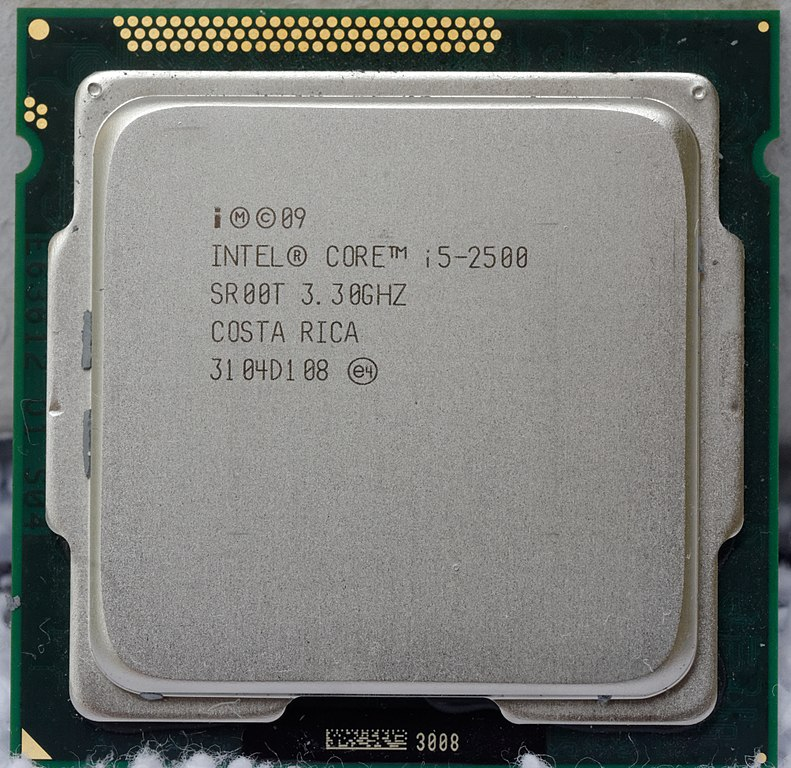
\includegraphics[width=.7\linewidth]{chapters/chp3/images/intel-i5-2500-processor.jpg}
        \caption{Um processador Intel\textsuperscript{\textregistered} 2500 \cite{wiki:i5_2500}.}
        \label{subfig:processor-example-1}
    \end{subfigure}
    \begin{subfigure}{.5\textwidth}
        \centering
        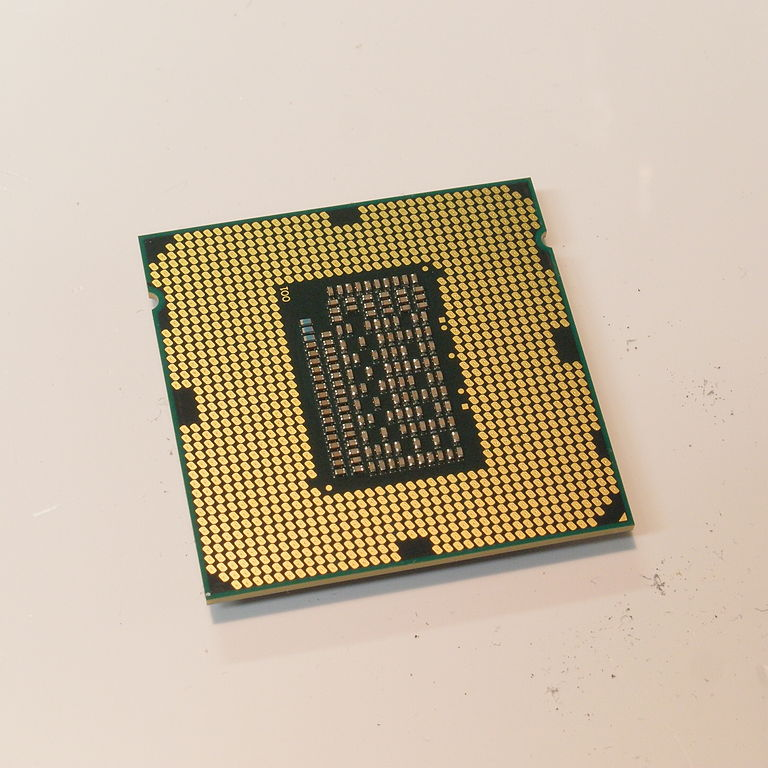
\includegraphics[width=.7\linewidth]{chapters/chp3/images/intel-i7-2600k-processor-pins.jpg}
        \caption{Os pinos de um processador Intel\textsuperscript{\textregistered} 2600 \cite{wiki:i7_2600}}
        \label{subfig:processor-example-2}
    \end{subfigure}
    \caption{Exemplos de processadores}
    \label{fig:processors}
\end{figure}
	    
    \section{A Memória Principal}

Quando se fala sobre memória computacional, pode-se estar referindo à memória 
cache, \acrfull{ROM}, \acrfull{RAM} ou à capacidade de armazenamento de um disco rígido. 
Dentre essas, a \acrshort{RAM} é considerada a principal e um exemplo dela 
pode ser visto na Figura \ref{fig:ram}. Ela é responsável por 
armazenar os programas em forma de processos gerenciados pelo sistema operacional, ou seja, 
enquanto eles estão sendo executados. Ela também é responsável por armazenar todos os dados 
gerados por um programa que ainda não foram ou descartados, ou salvos em disco ou cujo acesso 
ainda é requisitado.

Outras características sobre a \acrshort{RAM} são: 
\begin{itemize}
    \item o fato de que ela apenas armazena os dados até ser desligada, o que a classifica 
    como memória volátil;
    \item sua capacidade de armazenamento, que, na maioria dos casos, é maior do que a de memórias 
          cache e menor do que a de discos rígidos;
    \item sua velocidade, que segue o inverso da capacidade de armazenamento, ou seja, é menor do 
          que a de memórias cache e maior do que a de discos rígidos.
\end{itemize}

\begin{figure}[H]
    \centering
    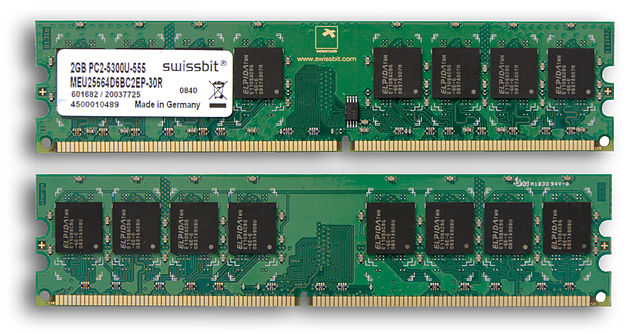
\includegraphics[scale=1.5]{chapters/chp3/images/Swissbit-2GB-PC2-5300U-555.jpg}
    \caption{Dois módulos de \acrshort{RAM} Swissbit\textsuperscript{\textregistered} 
    PC2-5300 DDR2 com capacidade de 2 Gigabytes, utilizada em computadores de mesa \cite{wiki:ddr2_ram}.}
    \label{fig:ram}
\end{figure}
	    
    \section{A cache}

    \begin{itemize}
        \item O princípio da localidade no tempo e no espaço;
        \item A necessidade da existência de uma cache, visto o 
        princípio da localidade;
        \item Explicação do que é uma cache;
    \end{itemize}
    
    \chapter{Disco rígido}

    \begin{itemize}
        \item O que são memórias voláteis e exemplos delas;
        \item A necessidade de memórias não-voláteis e o HD;
        \item Outras diferenças entre o HD e as outras memórias 
        envolvidas no trabalho
    \end{itemize}

	\section{Conseguir mais em menos tempo}

    \begin{itemize}
        \item A necessidade de se aumentar a velocidade de processamento;
        \item introdução aos problemas encontrados na computação serial
    \end{itemize}

    \subsection{A barreira da memória - \textit{Memory wall}}
    
        \todo[inline]{Conferir se existe mesmo a memory wall}
        \todo[inline]{Revisar o que é a memory wall e completar o itemize abaixo}
    
        \begin{itemize}
            \item 
        \end{itemize}
    
    \subsection{A barreira do paralelismo a nível de instruções - \textit{ILP wall}}
    
        \begin{itemize}
            \item Explicar do que se trata o paralelismo a nível de instruções;
            \item Explicar os conceitos de superpipeline e superescalar;
            \item Explicar que, ao se estender muito um pipeline, temos problemas;
            \item Explicar os problemas da superescalaridade
        \end{itemize}
    
    \subsection{A barreira no gasto de energia dos processadores - \textit{Power wall}}
    
        \begin{itemize}
            \item Introduzir a lei de Moore;
            \item Explicar que houve evolução na taxa de clock ao longo do tempo;
            \item Explicar que essa evolução foi amortecida nos últimos anos devido 
            ao gasto energético e às altas temperaturas que os processadores alcançaram 
        \end{itemize}
	
	\section{Paralelismo - a alternativa para se contornar as barreiras}

    \begin{itemize}
        \item Explicar no que consiste o paralelismo;
        \item em seguida, explicar porquê ele é uma saída possível
    \end{itemize}
    
    \subsection{Arquiteturas de memória na computação paralela}
    
        \begin{itemize}
            \item Explicar as arquiteturas:
            \begin{itemize}
                \item de memória compartilhada;
                \item memória distribuída;
                \item híbrida
            \end{itemize}
        \end{itemize}
    
    \subsection{Modelos da computação paralela}
    
        \todo[inline]{Conferir se serão esses modelos a serem apresentados}
    
        \begin{itemize}
            \item Shared Memory Model;
            \item Threads Model;
            \item Distributed Memory / Message Passing Model;
            \item Data Parallel Model;
            \item Hybrid Model
        \end{itemize}
    
    \subsection{Desenhando programas paralelos}
    
        \todo[inline]{ler a respectiva seção e completar aqui}
    
        \begin{itemize}
            \item 
        \end{itemize}